\section{Multi user chat server using TCP}
\subsection{Aim}
To implement a multi user chat server using TCP as transport layer protocol.

\subsection{Theory}
\textbf{TCP (Transmission Control Protocol)} works with the Internet Protocol (IP),
which defines how computers send packets of data to each other. Together, TCP
and IP are the basic rules defining the Internet. It is a connection-oriented protocol,
which means that a connection is established and maintained until the application
programs at each end have finished exchanging messages.\\
\textbf{Server} - In a simple multi user chat system, the server usually has the role to
receive the messages sent by the clients and send it to all other clients. So basically,
he handles the routing of the messages sent by one client to all the other clients.\\
\textbf{Client} - The client here acts from the side of the user. He sends the messages
to the server, and the server sends this message to all the other clients to simulate
a simple multi-user chat system.

\subsection{Algorithm}
\subsubsection{Server}
\begin{verbatim}
1 START
2 Create the TCP socket
3 Configure sockaddr_in struct
4 Bind the address struct to the socket using bind()
5 Accept incoming connections using accept()
6 Create child processes for these connections
7 Let these child processes handle each connected client
8 Until the termination of infinite loop repeat steps 8 - 10
9 Receive the data using recvfrom()
10 Send response using sendto()
11 Print the recieved data
12 STOP
\end{verbatim}

\subsubsection{Client}
\begin{verbatim}
1 START
2 I f argc <2(no a d d r e s s was pa s sed ) , ask for a d d r e s s and e x i t
3 C rea te the s o c k e t u si ng s o c k e t ( )
4 Configure sockaddr_in struct
5 Connect the socket to server using function connect()
6 Send the message to the server using sendto()
7 Recieve the response from server using recvfrom()
8 Print the response
9 STOP
\end{verbatim}

\subsection{Source Code}
\subsubsection{Server}
\begin{lstlisting}[language=C]
#include "message.h"
#include <errno.h>
#include <netinet/in.h>
#include <pthread.h>
#include <stdio.h>
#include <stdlib.h>
#include <string.h>
#include <sys/socket.h>
#include <sys/types.h>
#include <unistd.h>

#define MAX_CLIENTS 10
#define QUEUE_LENGTH 5

extern int errno;
const int PORT = 3000;

typedef struct sockaddr sockaddr_t;
typedef struct sockaddr_in sockaddr_in_t;

typedef struct
{
  int *client_fds; // Array of client fds
  int i; // Index of current client
  int *n; // Total number of clients
} thread_args_t;


void create_socket(int *socket_fd) {
  if ((*socket_fd = socket(AF_INET, SOCK_STREAM, 0)) == -1) {
    perror("Failed to create socket");
    fprintf(stderr, "Errno: %d\n", errno);
    exit(EXIT_FAILURE);
  }

  printf("Socket created successfully\n");
}

void configure_socket(const int *socket_fd) {
  sockaddr_in_t server_addr;

  server_addr.sin_family = AF_INET;
  server_addr.sin_addr.s_addr = htonl(INADDR_ANY);
  server_addr.sin_port = htons(PORT);

  if (bind(*socket_fd, (sockaddr_t *)&server_addr, sizeof(server_addr)) == -1) {
    perror("Failed to bind socket configuration");
    fprintf(stderr, "Errno: %d\n", errno);
    exit(EXIT_FAILURE);
  }

  printf("Socket binding successful\n");
}

void listen_for_client(const int *socket_fd) {
  if (listen(*socket_fd, QUEUE_LENGTH) == -1) {
    perror("Listening failed");
    fprintf(stderr, "Errno: %d\n", errno);
    exit(EXIT_FAILURE);
  }

  printf("Server listening\n");
}

void* recieve_message_from_client(void *args) {
  thread_args_t thread_args = *((thread_args_t *)args);
  message_t message;

  while(recv(
    thread_args.client_fds[thread_args.i], 
    (void *)&message, 
    sizeof(message), 0) > 0) {
    for(int i = 0; i < *(thread_args.n); i++) {
      send(
        thread_args.client_fds[i],
        (void *) &message,
        sizeof(message),
        0
      );
    }
  }
}

void accept_client(const int *socket_fd, int *client_fds, int *n, pthread_t *client_threads) {
  int client_socket_fd;
  sockaddr_in_t client;
  socklen_t len = sizeof(client);
  thread_args_t thread_args;

  if ((client_socket_fd = accept(*socket_fd, (sockaddr_t *)&client, &len)) ==
      -1) {
    perror("Accepting connection failed");
    fprintf(stderr, "Errno: %d\n", errno);
    exit(EXIT_FAILURE);
  }

  printf("Server accepted client %d\n", *n);

  thread_args.client_fds = client_fds;
  thread_args.n = n;
  thread_args.i = *n;

  client_fds[*n] = client_socket_fd;
  pthread_create(
    &client_threads[*n], 
    NULL, 
    (void *)recieve_message_from_client,
    (void *) &thread_args
  );
}



void main() {
  int socket_fd;
  int client_fds[MAX_CLIENTS];
  int n = 0;
  pthread_t client_threads[MAX_CLIENTS];

  create_socket(&socket_fd);
  configure_socket(&socket_fd);
  listen_for_client(&socket_fd);
  while(1) {
    accept_client(&socket_fd, client_fds, &n, client_threads);
    n++;
  }
    
  }
\end{lstlisting}

\subsubsection{Client}
\begin{lstlisting}[language=C]
#include <stdio.h>
#include <stdlib.h>
#include <sys/types.h>
#include <sys/socket.h>
#include <netinet/in.h>
#include <arpa/inet.h>
#include <errno.h>
#include <unistd.h>
#include <string.h>
#include <pthread.h>
#include "message.h"

extern int errno;
const int PORT = 3000;

typedef struct sockaddr sockaddr_t;
typedef struct sockaddr_in sockaddr_in_t;

static char username[USERNAME_LENGTH]; 

void create_socket(int *socket_fd) {
  if((*socket_fd = socket(AF_INET, SOCK_STREAM, 0)) == -1) {
    perror("Failed to create socket");
    fprintf(stderr, "Errno: %d\n", errno);
    exit(EXIT_FAILURE);
  }

  printf("Socket created successfully\n");
}

void connect_server(int *socket_fd) {
  sockaddr_in_t client_addr;

  client_addr.sin_port = htons(PORT);
  client_addr.sin_addr.s_addr = inet_addr("127.0.0.1");
  client_addr.sin_family = AF_INET;

  if(connect(
    *socket_fd, (sockaddr_t *)&client_addr, sizeof(client_addr)
  ) == -1) {
    perror("Failed to connect to socket");
    fprintf(stderr, "Errno: %d\n", errno);
    exit(EXIT_FAILURE);
  }

  printf("Connected to socket\n");
}

void send_message(void *args) {
  int socket_fd = *((int *) args);
  message_t message;
  strcpy(message.username, username);
  char message_text[MESSAGE_LENGTH];
  printf("To send a message type your message and press Enter\n");

  while(1) {
    scanf("%*c%[^\n]", message_text);
    strcpy(message.message, message_text);
    send(socket_fd, (void *)&message, sizeof(message), 0);
  }
}

void recieve_message(void *args) {
  int socket_fd = *((int *) args);
  message_t message;

  while(1) {
    while(recv(socket_fd, (void *)&message, sizeof(message), 0) > 0) {
      if(strcmp(message.username, username)) {
        printf("%s: ", message.username);
      } else {
        printf("You: ");
      }

      printf("%s\n", message.message);
    }
  }
} 

int main() {
  int socket_fd;
  pthread_t read_thread, recieve_thread;

  printf("Choose a username: ");
  scanf("%s", username);

  create_socket(&socket_fd);
  connect_server(&socket_fd);
  
  pthread_create(
    &read_thread,
    NULL,
    (void *) send_message,
    (void *) &socket_fd
  );

  pthread_create(
    &recieve_thread,
    NULL,
    (void *) recieve_message,
    (void *) &socket_fd
  );

  pthread_join(read_thread, NULL);
  pthread_join(recieve_thread, NULL);


  return 0;
}
\end{lstlisting}

\begin{center}
	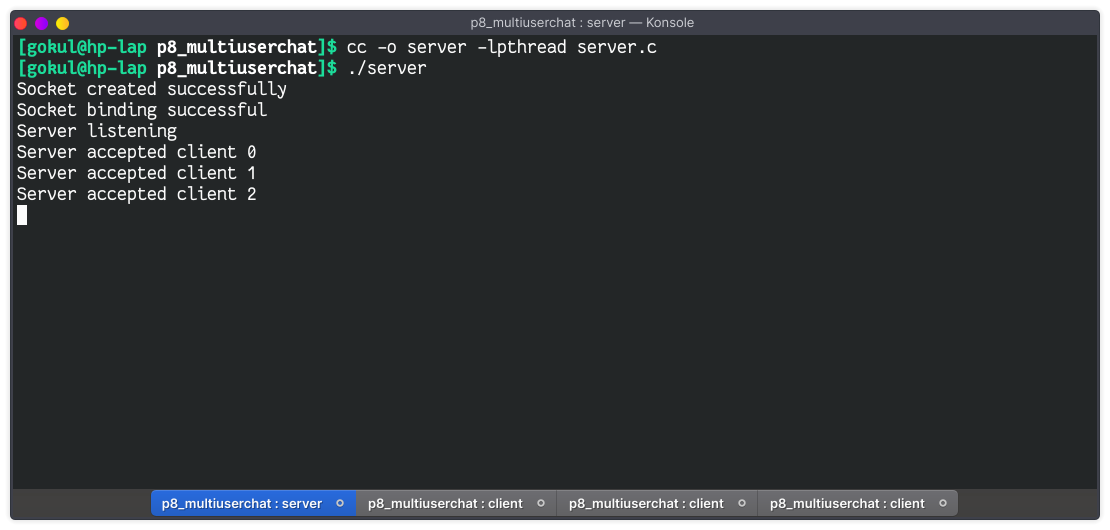
\includegraphics[width=0.90\textwidth]{img/p9/ss1.png}
	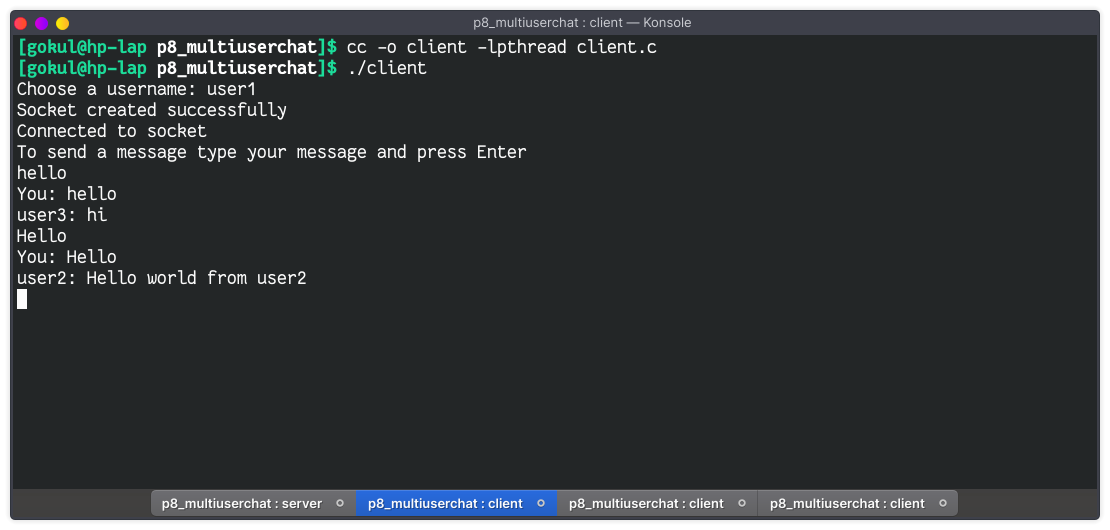
\includegraphics[width=0.90\textwidth]{img/p9/ss2.png}
	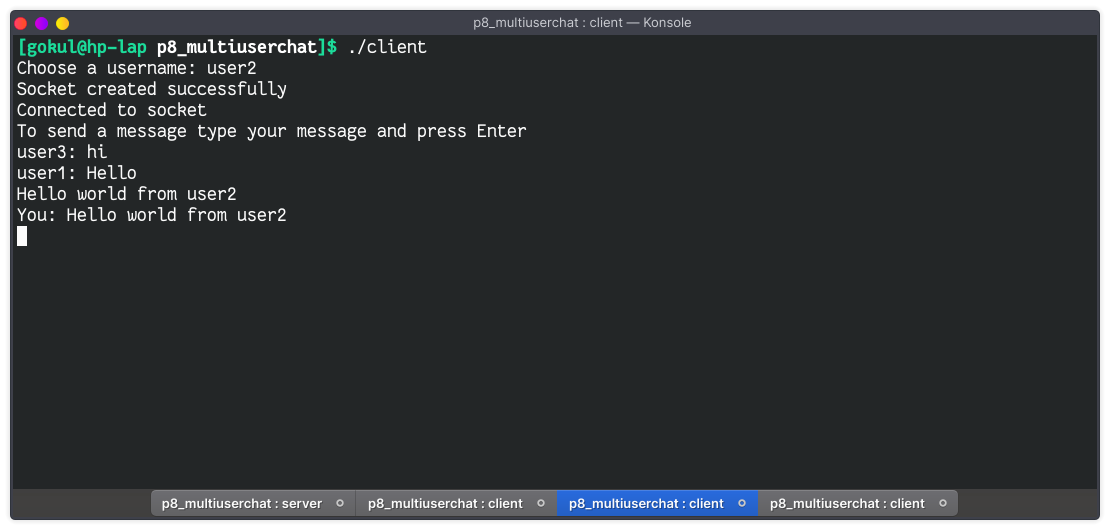
\includegraphics[width=0.90\textwidth]{img/p9/ss3.png}
	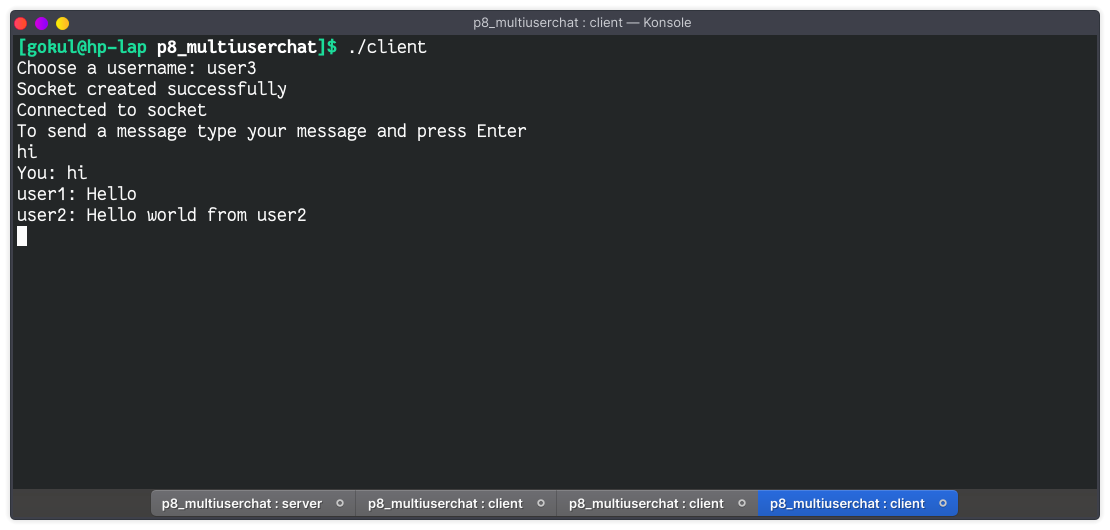
\includegraphics[width=0.90\textwidth]{img/p9/ss4.png}
\end{center}


\subsection{Result}
The above programs were executed and its output were verified